% using LuaLaTex

%\documentclass[a4paper,12pt,twoside,draft]{book}
\documentclass[a4paper,10pt,oneside]{book}
\usepackage[nokeyprefix]{refstyle}
\usepackage[toc,page]{appendix}
\usepackage[fleqn]{amsmath}
\usepackage{mathdots}
%\usepackage[utf8]{inputenc}
\usepackage{graphicx}
\usepackage{makeidx}
\usepackage[nounderscore]{syntax}
\usepackage{url}
\usepackage[pdfpagelabels=true,plainpages=false,hyperfootnotes=false]{hyperref} % last package!

% On Fingures and floats see: https://en.wikibooks.org/wiki/LaTeX/Floats,_Figures_and_Captions

% TeXstudio: This comment block is for TeXstudio users only, it is not essential for building the documentation and provides a way to copy the pdf to a more convenient location.
% TeXstudio: see: https://tex.stackexchange.com/questions/187672/path-for-saving-pdf-in-texstudio
% TeXstudio: This only works if
%            1) you are using TeXstudio
%            2) have added the user command [copyPdf:Copy Pdf][cmd /C copy %.pdf ..] in Options -> Config TeXstudio -> Build -> User Commands (with command detaild for windows).
% TeXstudio: To copy pdf result to target location use Tools -> User -> Copy Pdf

\newcommand{\GS}{LaserGrayscales}
\author{A.H.M. Steenveld.}
\title{
    \begin{figure}[h!]
        \centering
        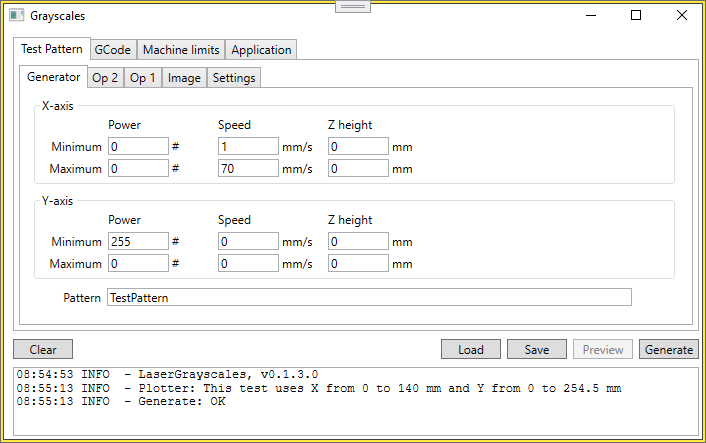
\includegraphics[width=0.8\linewidth]{./images/Grayscales-v0.1.3.png}
    \end{figure}
    The \GS\ test generator.
}
\date{November 2024}

\bibliographystyle{plainnat}

\newcommand{\Warning}[1]{\begin{quote}\textbf{Warning}: \emph{#1}\end{quote}}
\newcommand{\WarningCheckAndTest}{\Warning{Always test and check a script before using it.}}

\mathchardef\mhyphen="2D

%\parindent=0pc			    % Do not indent the start of a paragraph.
%\setlength{\parskip}{1pc}	% Put an empty line between paragraphs.
\flushbottom				% Size all pages to the same length.

% syntax setting.
\setlength{\grammarindent}{7.5em}
\newcommand{\grammarltgt}[1]{\textless#1\textgreater}
\newcommand{\grammarnl}{\grammarltgt{newline}}

\makeindex\pagestyle{empty}
\begin{document}
    \maketitle\frontmatter\maketitle%
    \chapter{Introduction}\label{Introduction}

\GS\ is a tool to test the effects of your laser at power levels 1 through 255 and
at speeds ranging from 1 mm/s to 70 mm/s or 60 mm/min to 4200 mm/min and different
Z heights. This is a good way to see how your laser will react to different materials
at different speeds and power levels.

\GS\ was started `out of necessity' of having no proper test tools for a new laser
engraver tool. On the internet a \href{https://www.thingiverse.com/thing:3349071}{g-code script}
is available but its use of g-code is targeting different elements of the industry
standard RS274 format than what was acceptable for the g-code interpreter with my machine.
Changing the script manually was time consuming and just for one script where more testing
is required.

\GS\ works on the idea that you want to display the same image using different settings
for speed, laser power and Z height. You can plot an image `X' one time then change the settings
and plot it again (and again). \GS\ let you plot a line of images `X' `X'... `X' and specify
a different setting for each image. And it can do that for multiple lines. You also have
control over the amount white space between images and lines and between group of
images and group of lines.

The `image' can be as simple as one straight line, a box (without any filling in it), a square
with an uniform grey filling or an image from file (yet to be implemented).

This allow you to make a crude first try to look for the sweet spot you need and then
to refine limiting the range and making smaller steps to find the best settings for your
application.

    \tableofcontents\mainmatter%
    \chapter{Quick start}\label{QuickStart}

Starting \GS\ for the first time you get an opening screen. And then?
This will give you a quick introduction to get started with some suggestions on how to use it but without explaining too much. All the explaining is done in subsequent chapters.
For full details on all screen details, buttons and text see chapter \nameref{ScreensMenuButtons}. buttons'%\Chapref{Screens, menu and buttons}'.

\begin{figure}[h!]
    \centering
    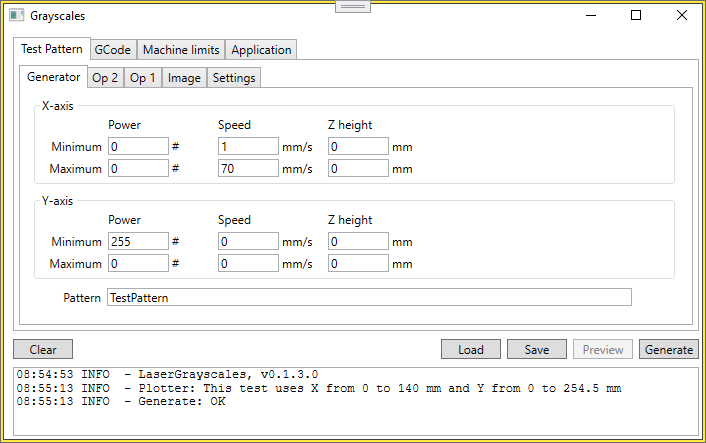
\includegraphics[width=0.8\linewidth]{./images/Grayscales-v0.1.3.png}
\end{figure}

\section{Configuration}
Starting for the first time a configuration for `Stepcraft, D3/600' using `UCCNC' is assumed.

If you are not using a `Stepcraft, D3/600' machine see the tab `Machine limits' and check that the limit settings comply with your machine. Change settings accordingly. This needs to be done only once.

If you are not using `UCCNC' as GCode interpreter see the tab `GCode' and check that configured GCode comply with your interpreter. Change settings accordingly. This needs to be done only once.

You can skip these first two steps and still generate test patterns but the GCode for it might well be violating your machine limits or be invalid for your interpreter. This also might be the case
if you do make the first to steps but made some errors or oversights.

\WarningCheckAndTest

\section{Test script}
The default test script is set for an image of 0 to 140 mm on the X-axis and 0 to 255 mm on the Y-axis, Z is fixed at 0 mm.

The image is 255 continues lines in the X direction, separated by 0.5 mm in the Y direction.
In the X direction speed (for G1) is changed from 1 to 70 mm/sec (60 to 4200 mm/min) and in the Y direction laser power is changed from 255 (100\%) to 0 (0\%).

In the tab `Image' you see details for the line segments, by default a line segment (written at a fixed speed an laser power) is 2 mm long (in the X direction) and the next line (in the Y direction)
is 0.5 mm above it. These two settings have a major influence on the final width and height of the image and also on that what you want to test. In stead of lines you can also use squares, blocks or images.

In the tab `Op 1' (for Operation 1) you see that in the X direction there is no gap between the images and that it is repeated 70 times. In the Y direction there is an additional gap 0f 0.5 mm.
Tab `Op 2' is similar and defines one image (no repeats) and defining a gap here does not do anything.

To arrange grouping of 8 lines one can define an Image count of 8 in the y direction on the `Op 1' tab and an Image count of 32 in the y direction with an appropriate gap on the `Op 2' tab.

At the `Generator' tab the settings for Power, Speed and Z-height for each image is defined. This is done for both the X direction and the Y direction. The actual value used is the sum of both.
By default the Z-height is at a constant value of 0.

The speed is changed van 1 to 70 mm/s (60 to 420 mm/min) in the X direction. There are 70 line segment images in the X direction thus each
image in the X direction is done 1 mm/sec (60 mm/min) faster than the previous one.

The laser power is changed from 0 to 255 in the Y direction. There are 255 lines in the Y direction thus each image in the Y direction is using one step of laser power more than the previous one.

The text field `Pattern' is used for the name of the generated pattern. This name is appended with a date/time stamp.

\section{Generating a script}
After checking all settings it is time to generate the test script. Press the button `Generate' and a script is written to `.\textbackslash{}build\textbackslash{}TestPattern-yyyy-MM-ddTHH.mm.ss.nc'

With the `Save' button you can save all your test settings in a file, with `Load' you can load it again. The button `Preview' is for future use.

At the bottom of the form you can follow the progress of generating the script and look at some details for invalid values. Generating the standard script with lines will take a few seconds
depending on PC capabilities. It is reasonable to expect something at or below 10 seconds, a time of one minute is unrealistic long.
%When using the same settings for a standard script and apply it to a square it will take a prohibitive amount of time (and memory). Try a small pattern first and see how fast how many lines
%it generates. Progressively make it bigger until you get what you need or when time, memory or lines become unacceptable large.

\section{Reducing script processing time}
Executing the GCode from the default script takes a lot more time and a lot of material, both considerd to be scarce resources. On a Stepcraft D3/600 a processing time of around one hour is
to be expected. A surface of 140 x 255 mm of some (possible expensive) material does not feel right either. With common sense there are several options to reduce this time. The script is
configured to take one unit step for speed and laser poser and run over the full scale of it.

First suggestion is not to run over the full scale but only over the part that is about right, say a speed of 30 to 60 mm/sec  (1800 to 3600 mm/min) and a laser power range of 100 to 200
(about 40\% to 80\% of full laser power). That on its own is not sufficient. Also reduce the number of copies in `Op 1' (and in `Op 2' if you are using it) to a total of say 10 in each direction
This will give a big reduction is processing time bringing it back to the range of minutes. But it also produce a more coarse result. With this result you may be able to select the rough settings
of speed an laser power for an optimal result and generate a second test around these values.

This way it is possible to get good estimates of settings using a minimum abound of time and material.

    \chapter{Principles of operation}\label{PrinciplesOfOperation}

The program can be used to generate test patterns to find the sweet spot of operations for a particular image on some
material. It is also possible to create test patterns for testing the CNC hardware or the laser equipment up to a point.

To get the maximum out of \GS\ it helps to understand how it works. Not in terms of buttons and values but in how it was
designed and how information is used to produce test patterns.

The program applies a number op operations on an initial image\index{image}\index{image!initial}.
Each operation\index{operation} generates a new image. The last operation is producing G-Code for a test pattern.
Operations before that may apply a repeat pattern on the image or put a border around the image. It will be relatively
easy to implement a new operation at a later time.

For a first version of \GS\ a limited number of operations in a fixed order will be available. Giving the user more
flexibility in the order of applying operations is for a future version. The same for the initial images, a limited
number of initial images will be available. In future versions more types of images will become available.

There are a number of arguments that can be changed during the test, collectively called the
`{arguments under test}'\index{argument under test}.
When generating a test a original image\index{image!original} is repeated a number of times and each image will use
different and specific values for the arguments under test. Available for arguments under test are Z
height\index{argument under test!Z height}, speed\index{argument under test!speed} and
laser power\index{argument under test!power}.

\section{Design requirements}
A number of requirements were formed early for \GS.
\begin{itemize}
    \item Test patterns must always operate within target machine capabilities.
    \item Designing a test pattern must be possible for many G-Code consumers, not for just one machine or manufacturer.
    \item Produced G-Code must be minimal and adhere as much as possible to RS274-D.
    \item Generating G-Code must be  as fast as possible (in seconds, not in minutes).
    \item New users must be able to construct a test pattern safely without much concerns about how to use the program
          (low learning curve, result examples) but not hinder the experienced user (efficient user input).
    \item While configuring a test pattern it must give an indication where target machine capabilities are
          causing clipping of arguments under test on the image.
    \item While configuring a test pattern it must immediately indicate its size in x and y directions.
    \item While configuring a test pattern it must give a run time indication.
    \item The start point of a test pattern is an image to be realised with some arguments under test.
    \item Arguments under test include:
          \begin{itemize}
              \item Z height while engraving (for `out of focus' effects).
              \item Speed while engraving (for speed versus power effects).
              \item Intensity of laser while engraving (for speed versus power effects).
          \end{itemize}
    \item A number of operations must be available on the image including:
          \begin{itemize}
              \item Limits operator: All values used by the (final) image are within the capabilities range of the
                    target machine all the time.
              \item Pattern operator: The (final) image must be repeated first in X direction and then in Y direction.
              \item Border operator: The (final) image is given a border with some raster information.
              \item Rotation operator: The (final) image can be rotated  over any angle.
              \item Translation operator: The (final) image can be moved to any position
          \end{itemize}
    \item Operations must be repeatable e.g.: applying the Pattern operator twice will create an outer pattern over
          an inner pattern over an image.
\end{itemize}

\section{Images}
There is an image\index{image|textbf} to start with. This is the `original image' and the intension is to repeat it
several times and test it with different settings.

All images have is a width and an height. A number of images are available, more are in the planning.
Each image have some intended use. Each image have a specific purpose in mind. For each image some typical setting ranges
are given. These ranges are not mandatory but just sensible ranges for values to begin with. If the results are not good
do try some values outside the advised ranges.

\subsection{The line}
The purpose of the line\index{line|see {image}}\index{image!line} is to see the effects of some setting. It is the basis
of all testing.
On its own it does not give much information but chaining a number of lines in a row where all lines are the same but
for one the gradual effects of that one setting changing over the full length  will show the effect more clearly.
A next line above the first one  allows for a second setting to check the combined effect of two settings in an easy way.

Line lengths are defined in the x direction by setting the width. The typical setting falls in the range of 5 mm to 20 mm.
A line width is not defined. Note: The width is defined by the laser spot, very small and may be depending on how the laser
equipment is mounted if the spot is not round. In most cases it is a relative long and in the middle thin elliptic shaped.

Space between lines in the y direction are defined by setting the height. A typical setting is in de range of 0.25 mm to 0.5 mm.

\subsection{The box}
The purpose of the box\index{box|see {image}}\index{image!box} is to see the effect of laser power in the lower ranges
at higher speed.

A box is defined by four lines along its side. There is no filling in the box. A typical setting for width and height
is in the range of 50 to 100 mm. For higher speeds larger settings give better results.

While the G-Code interpreter is executing blocks of commands it has a few things to take care for. One is stopping at
(sharp) corners. When it is getting near a corner it must stop moving in one direction and start moving in another one.
This will take time and deviations from the selected speed.

Some G-Code interpreters will keep the laser at constant power all the time but others might be adaptive and when
decelerating for the corner also lower the laser power.

Lasers have the property that below some power\index{argument under test!power} threshold level they will not fire,
there is just not enough power to emit any light. Finding that level where the laser is guaranteed to fire is an
important step for getting good and consistent result.

Running a test with a box can produce tree results.
\begin{enumerate}
    \item The line ends at the corners are more black than in the middle.
    \item The line ends at the corner are equally black as in the middle.
    \item The line stops before it is at the corner.
\end{enumerate}

In the first case the conclusion is that the G-Code interpreter is not adaptive. Lower speeds result in more blackness.
Try to work with lower speeds in your project to reduce the effects of this.

In the second case the results are fine. The G-Code interpreter may or may not be adaptive. The settings for speed an
power are useful and give good results.

In the third case the G-Code interpreter is adaptive and is lowering the laser power below the threshold point of the
laser. Again, try to lower the speed to reduce the effects of this. Also, try to find out what the threshold level of
the laser is so you can keep that in mind when selecting a power level.

\subsection{The square}
The purpose of the square\index{square|see {image}}\index{image!square} is to see the effects of engraving a surface.

A square is defined as a box with a filling in lines per cm in it. Typical settings for width and height fall in the
range of 5 mm to 100 mm. Typical settings for lines/cm are 20 lines/cm to 50 lines/cm. (higher settings will increase
processing time proportionally.)

Typically when engraving a line it has a length and nearly any width. The laser is in focus and ideally all the laser
light is in one spot. This might result in an engraving with many visible lines, like an old copper engraving print.
This might or might not be the result to achieve. Raising Z up to a few mm will soften the lines. Lowering might give
the same results but with the effect that the laser equipment is getting nearer to the surface.

One way of softening this effect is getting the laser out of focus by raising the Z height\index{argument under test!Z height}
(and maybe raising the power to keep in check with the grey level) There is no measurable good or bad result for this
test, it all depends on the desired effects but this test give some more control over the end results.

\subsection{The card}
(Not yet implemented.)

The intention of the card\index{card|see {image}}\index{image!card} is to have a small representative part of the end
result and do a test run with it. There is no measurable good or bad result, it serves more as a check around the
selected settings for fine tuning or as a final check.

Once this test is available the it will also be possible to engrave the full image. Except that the software for
engraving at some speed and power settings might also have some operations on image manipulating such as sharpening,
softening, despeckle, gamma correction and more.

\section{Operations}
A limited set of operations is available. As a matter of fact only two and one is automatic applied. The other one
can be applied zero, once or two times. More operations and more freedom on applying or not is in development.

Each operation\index{operation}, except for the generator operation will result in a new image where the original
image is part once or more times. The generator operation creates a G-Code file.

\subsection{The Pattern}
The intention of the pattern%
\index{pattern|see {operation}}\index{operation!pattern}
is to repeat an image in x and y
direction with no or some space between all images.

Each image copy is numbered with grid coordinates, on the x axis running from (0, y), (1, y) ... (n, y) and similar
on the y axis from (x, 0), (x, 1) ... (x, m). The grit numbering is fixed and other operations will not change it.

Repeated pattern operations will result in multiple levels of coordinates and each original image\index{image!original}
will have a unique address. The unique address of an original image and the total count of original images on
the x axis (or y axis) is used to calculate values for arguments under test.

\subsection{The Grid and border}
(Not yet implemented.)

\subsection{The Rotation}
(Not yet implemented.)

The purpose of this operation is to rotate the image over a number of degrees at its centre.

\subsection{The Translation}
(Not yet implemented.)

\subsection{The G-Code generator}
Technically this is an operation\index{generator|see {operation}}\index{operation!generator} and it is applied as
the last operation. The results are not another image but a G-Code file.

This operation have several tasks.
\begin{itemize}
    \item Calculate values for arguments under test with each original image.
    \item Check and clip all values against target machine minimum and maximum values.
    \item Generate G-Code file suited to the target machine.
    \item Write G-Code to file.
\end{itemize}

\paragraph{Calculating values for arguments under test.}~\\
At this phase the maximum number of original images in x and y direction is calculated. Then for each
original image\index{image!original} the values for the arguments under test are calculated.

All images in the x or y direction may or may not be all in a straight line. X and y here are index numbers and not
positions on a XY plane. Rotating an image may result in direction changes but the numbering is not changed, e.g.:
rotating 90 degrees counter clockwise will result in the x numbering running in the y direction and the y numbering
in the -x direction. No corrections are made for this and values for arguments under test are applied as calculated
for the x and y value.

For each argument under test\index{argument under test} a value is calculated using the formula

\begin{equation}
    value_a = min_a + \frac{index_a}{index_{a, max}}(max_a - min_a)
\end{equation}

Where $a$ is $x$ or $y$, $min$ and $max$ are given limits by scale values and $index_a$ and $index_{a,max}$ depend on
position and number of original images in a given direction.

Then $value_x$ and $value_y$ are added together, this sum is used as the value for the argument under test for the
image with index $(x, y)$.

Example: Speed values is scaled in the X direction as $(0, 0)$ and in the Y direction as $(20, 50)$. Power values is
scaled in the X direction as $(100, 200)$ and in the Y direction as $(0, 0)$ and there are 10 original images in the
x direction and 4 in the y direction.

Then the speed (in mm/sec) and power value for image with index $(3, 2)$ is:
\[ speed_{x} = 0 + \frac{3}{10}(0 - 0) = 0 \]
\[ speed_{y} = 20 + \frac{2}{5}(50 - 20) = 32 \]
\[ speed = 32 \]
~\\
\[ power_{x} = 100 + \frac{3}{10}(200 - 100) = 160\]
\[ power_{y} = 0 + \frac{2}{5}(0 - 0) = 0\]
\[ power = 160 \]

One thing to notice is that it is possible to have scaled values for arguments under test in both X and
Y direction. The two will be added together and the results will be a skewed setting on the XY plane for that
argument under test.

\paragraph{Check and clip.}~\\
\index{clip}Before G-Code is generated all calculated values are checked against machine limits\index{machine limits}.
For configuring machine limits see the chapter on configuration details.

Each and every calculated value\index{calculated value} is checked against a minimum value and a maximum value.
If the calculated value is less than the minimum value then it is replaced by the minimum.
If the calculated value is greater then the maximum value it it replaced by that.

\Warning{It is not guaranteed that all values used are within machine limits\index{configuration!machinesettings}.
There are user supplied sections for intro, header and footer. The user can inject values\index{inject values} out of range.}

\paragraph{Generate G-Code.}~\\
The next phase is to generate\index{operation!generator|textbf} G-Code from the final image. The G-Code is partitioned in several sections.
\begin{itemize}
    \item \GS\ information details.
    \item User supplied info section (copied verbatim, no processing done)
    \item Test pattern details, all settings supplied in the user interface as an overview.
    \item X and Y ranges used by the test pattern.
    \item G-Code settings required by the script.
    \item User supplied header section (copied verbatim, no processing done)
    \item G-Code for the test pattern
    \item G-Code to safely stop the script
    \item User supplied footer section (copied verbatim, no processing done)
\end{itemize}

The three user supplied sections are copied verbatim. No checking or other forms of parsing is done on it.
This may be a cause of problems. It is possible to inject values that are out of machine acceptable limits
or a comment form is used that is not supported by the G-code interpreter.

\WarningCheckAndTest

\paragraph{Write G-Code.}~\\
Building and generating a G-Code file uses a build area\index{build area}. Its location is configurable and by default
`.\textbackslash{}build'. Intermediate results are stored here if required and so is the final result.

\section{Arguments under test}
\index{argument under test|textbf}There are three values that can vary over a range of values.
The three being Z height\index{argument under test!Z height}\index{Z height|see {argument under test}},
speed\index{argument under test!speed}\index{speed|see {argument under test}} (for G1 codes)
and Laser power\index{argument under test!power}\index{power|see {argument under test}}.

Applied values range from a minimum value to a maximum value and are calculated linearly in X and Y direction
based on the number of original images\index{image!original} in each direction. The calculated values in X and Y
direction are added together and used as the final value.

On normal use a calculated value will have some scale in one direction and is constant in the other. Test patterns
using this configuration result in one argument changing from image to image in one direction and another one
changing in the other direction. Finding good or bad result is more or less checking a table.

It is possible for calculated values to have some scale in both directions. This can be useful if the normal use
will give skewed results. While skewing the scales in the other direction this can be compensated. Its use will
depend on specific test details.
    \chapter{Screens, menu and buttons}\label{ScreensMenuButtons}

What you get is what you see. A bunch of screens in multiple tabs. What you see is not exactly what you get in terms of test patters.
To understand what you get you must first understand what you see. This chapter is all about that. Step by step all screen, all fields
and all buttons get explained.

There might be small deviations in the images here compared to the actual program. Changes in the program are not always immediate
reflected in the documentation.

The main form (and up to now the only form) is using several tabs for configuration and creating test patterns. Each tab is
a screen on its own right and needs an explanation. The organisation of the tabs and this explanation is from the more detailed
to the more global subjects. Where the `Test Pattern' tab, `Generator' subtab gives a lot of details about generating a test pattern
the `Application' tab only give some settings to bind all the parts together. All in all it is not complicated, it is just a lot of details.

Advise to the reader: Skim trough this chapter before trying to read and understand all the details. If you have not yet done so read the
chapter \nameref{QuickStart}. Make a few test patterns to get a feel of how it all comes together before you zoom in on the particular test pattern
you want.

In the following paragraphs there screens are explained:
\begin{itemize}
    \item The startup screen.
    \item The Test pattern tab.
        \begin{itemize}
            \item The Generator sub tab.
            \item The Operation 2 and Operation 1 sub tabs.
            \item The Image sub tab.
            \item The Settings sub tab.
        \end{itemize}
    \item The GCode tab.
        \begin{itemize}
            \item The Settings sub tab.
            \item The Intro, Header and Footer sub tabs.
        \end{itemize}
    \item The Machine limits tab.
    \item The Application tab.
\end{itemize}

\section{The startup screen}\label{StartupScreen}
\begin{figure}[h!]
    \centering
    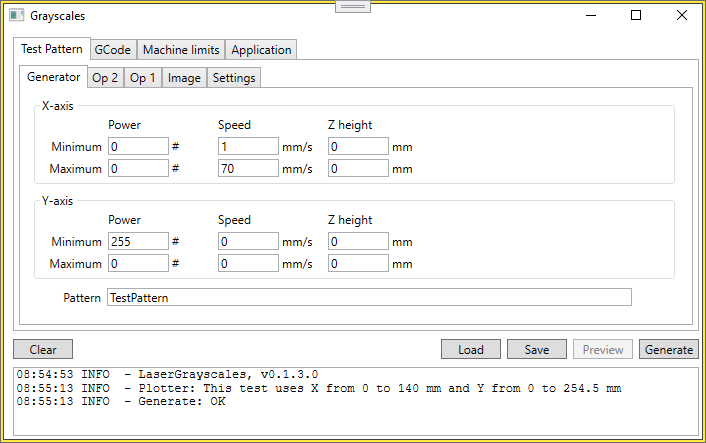
\includegraphics[width=0.8\linewidth]{./images/Grayscales-v0.1.3.png}
\end{figure}

This is the first screen you see when starting up. The top part has a tab selection for `Test Pattern', `GCode', `Machine limits' and `Application'. All these tabs
are explained in the following sections.

At the lower end of the form you see a row of buttons and below that some text.

The text part is functioning as a feed back to tell you what the program is doing and which problems have occurred. It is possible to clean this with the `Clear' button
on the left side above it.

The row of buttons include (from left to righ).
\begin{description}
    \item[Clear] To clear the text part below it.
    \item[Load]  To load a previously saved test pattern, replacing all settings in the `Test Pattern' tab.
    \item[Save]  To save a test pattern, write all settings in `Test Pattern' to file. A file name is suggested and you can change it before writing.
    \item[Preview] To get a preview image of the `Test Pattern' (not yet implemented).
    \item[Generate] To generate a G-Code file from the `Test Pattern' settings and taking in account the limits set for the GCode interpreter and the Machine.
                    The default location for the gcode file is `.\textbackslash{}build\textbackslash{}TestPattern-yyyy-MM-ddTHH.mm.ss.nc'. The name `TestPattern' is
                    taken from the text field `Pattern' in the `Test Pattern', `Generator' sub tab. A timestamp is appended to the name. After successfull generation
                    you are asked where to copy the result to.
\end{description}

\section{The Test Pattern tab}\label{TestPatternTab}
%\begin{figure}[h!]
%    \centering
%    \includegraphics[width=0.8\linewidth]{./images/Generating.png}
%\end{figure}

This is the tab where the layout of a test pattern is configured. It has a sub tab for generator settings, two sub tabs for operations on the image (in this version
the operations are fixed and both for arranging copies of the image), a tab for image settings and a final tab for some general settings. A description of each
sub tab is given below.

The test pattern is rectangle with a number of repeated images in the X and Y direction. Each image has a unique x and y coordinate where the coordinates start
with 1 and ends with a final number. Each image is uniquely identified by its $(x, y)$ coordinates.

Each image is drawn/plotted with a specific setting for speed, laser power and Z height. These three values (known as the `arguments under test') are calculated
based on the $(x, y)$ coordinates from the image, the values will always be within machine limits, underflow is replaced by the machine minimum value and overflow
is replaced by the machine maximum value.

\subsection{The Generator sub tab}\label{TestPatternGeneratorTab}
\begin{figure}[h!]
    \centering
    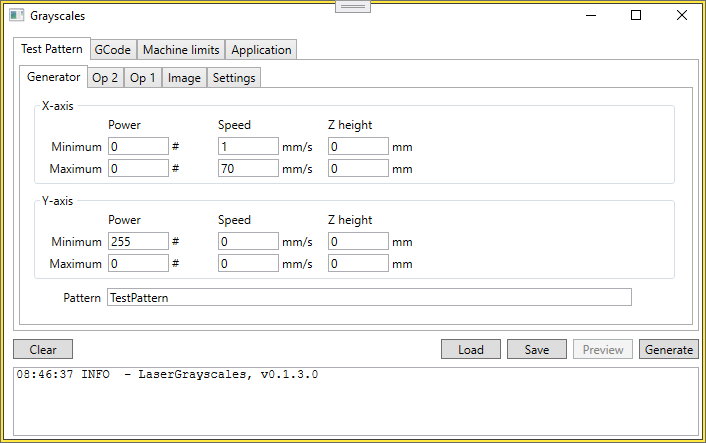
\includegraphics[width=0.8\linewidth]{./images/Generator.png}
\end{figure}

The `Generator' sub tab is for setting values that are used for generating the test pattern. It has three parts.

The first two are `X-axis' and `Y-axis' both with identical settings but obviously for a different axis. For each axis a range of settings for the three
`arguments under test' is defined. Values for X axis and Y axis are added together before using it to draw/plot the image.

It is possible to keep a value at a constant for all images, e.g.: to make the Z height constant at value 0 fill in a 0 for minimum and maximum on both the X and Y axis.

It is possible to change a value in one axis direction only, optionally with a fixed offset, e.g.: speed changing from 1 to 70 mm/sec (60 to 4200 mm/min) in the X direction
and with a fixed offset of 0 specified by the Y direction. It is possible to specify an offset in two (equally valid) ways. The first, as in the example before, is using one axis
for the variations and the other axis for the offset. The other way is to use one axis for both the offset and the variation and set the other axis to a constant value of 0, e.g.:
speed changing from 20 to 50 mm/sec with speed minimum set to 20 and speed maximum set to 50 on the X axis and a value of 0 for both speed minimum and speed maximum on the Y axis.

It is also possible to use different scales on both the X axis and the Y axis this will result in a skewed distribution of values used on the images. In the previous examples
all settings for speed in the Y direction for some index $y$ are identical which makes it easier to evaluate and select a good speed setting. With a skewed setting this is no
longer the case. The advantage of a skewed setting is that it is possible to test a setting over a wider range leaving out some less important combinations of `argument under test'
combinations.

The actual value for $(x, y)$ is calculated with the scale settings and the total number of images in the direction. The total number of images in a direction is depending on
settings for repeat in tabs `Op 1' and `Op 2'.
It is possible to specify a `minimum' value that is bigger than the `maximum' value. More correct names are `start value at the beginning of a sequence' and
`end value at the beginning of a sequence'. Given a total repeat number of $N$ in one direction the value used for index $n$ is `$minimum + \frac{n}{N}(maximum - minimum)$'.
See \nameref{PrinciplesOfOperation} for more details.

The field `Pattern' is used as the base name for the test pattern file generated. See also \nameref{StartupScreen}.

\subsection{The Operation 2 and Operation 1 sub tabs}\label{TestPatternOpTab}
\begin{figure}[h!]
    \centering
    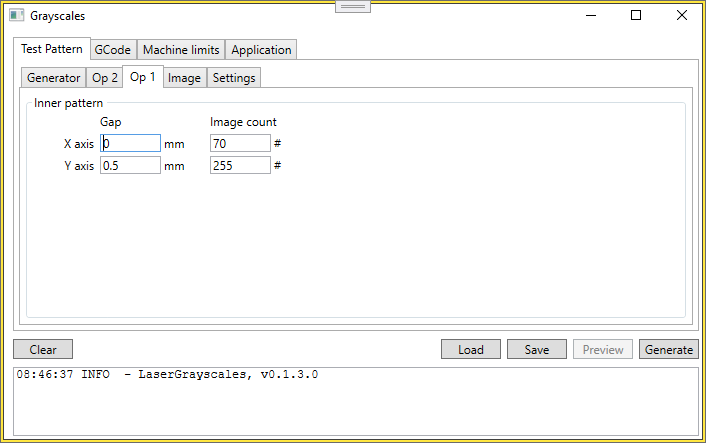
\includegraphics[width=0.8\linewidth]{./images/Operation1.png}
\end{figure}

The `Op 2' and `Op 1' tabs are identical again. Each one specifies a grouping operation in the X and Y direction. `Op 2' is applied before generating and after `Op 1'.
In the same sense `Op 1' is used by `Op 2' and is using `Image'. The name in the tabs used for `Op 2'  is `Outer pattern' en for `Op 1' it is `Inner pattern'.

The repeat pattern specifies a number of copies or `Image count' in the X and Y direction defining a rectangular of images. It also specifies free space or `Gap' in mm
between the repeated images. With the two repeating patterns it is possible to sub divide the final result in groups. This way it is easier for find the actual values
used for `parameters under test'. Note: with the border operation available it will be possible to write an index or value in the final result. This operation is
not yet available.

See \nameref{TestPatternGeneratorTab} for some examples on how to group images. See \nameref{PrinciplesOfOperation} for more details.

\subsection{The Image sub tab}\label{TestPatternImageTab}
\begin{figure}[h!]
    \centering
    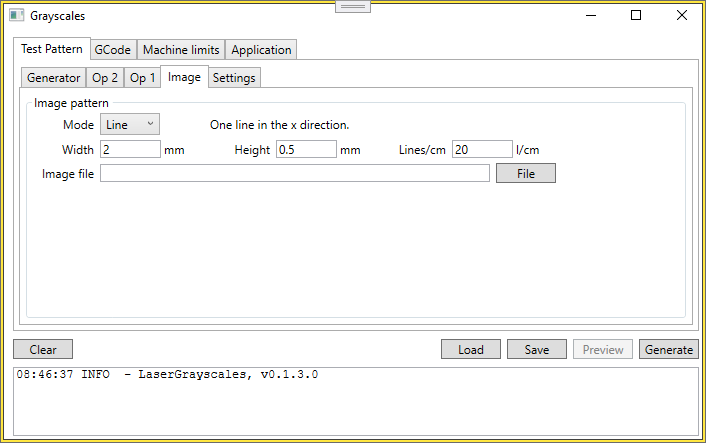
\includegraphics[width=0.8\linewidth]{./images/Image.png}
\end{figure}

In this tab the actual Image to draw in each copy is specified. A few settings are in use for it. An image is always a rectangular shape with a width and a height.
If the rectangle has a filling then the lines per cm is used otherwise it is ignored.

There are four shapes, called `Mode', of images possible.
\begin{description}
    \item[line]   A line at the lower end of the rectangle.
    \item[box]    Four lines, one at each side of the rectangle, no filling in the rectangle.
    \item[square] A box with a lines filling inside running in the x direction.
    \item[card]   A square with an image inside (not yet available).
\end{description}

For normal testing the `Line' mode will give you sufficient information to select the most appropriate settings for `parameters under test' in your application.
Each shape or `Mode' is designed to test some specific properties of the machine and interpreter configuration. See \nameref{PrinciplesOfOperation} for more details.

\subsection{The Settings sub tab}\label{TestPatternSettingsTab}
\begin{figure}[h!]
    \centering
    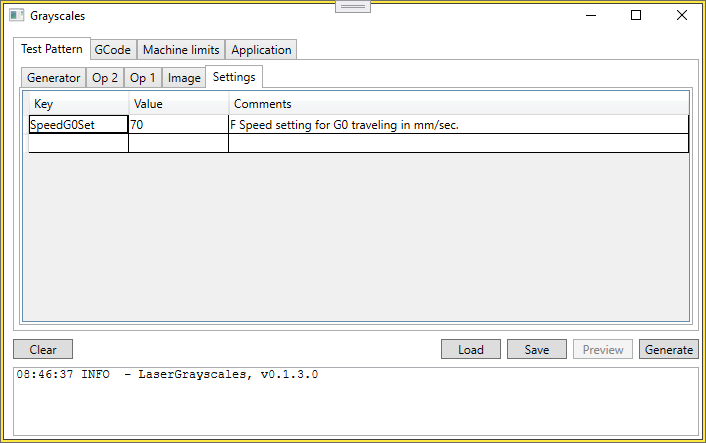
\includegraphics[width=0.8\linewidth]{./images/Settings.png}
\end{figure}

For the test pattern one setting is available. That is the speed (in mm/sec) available for `G0' gcode move actions. This value is limited by the GCode minimum and maximum settings,
see \nameref{GCodeSettingsTab}

\section{The GCode tab}\label{GCodeTab}
\begin{figure}[h!]
    \centering
    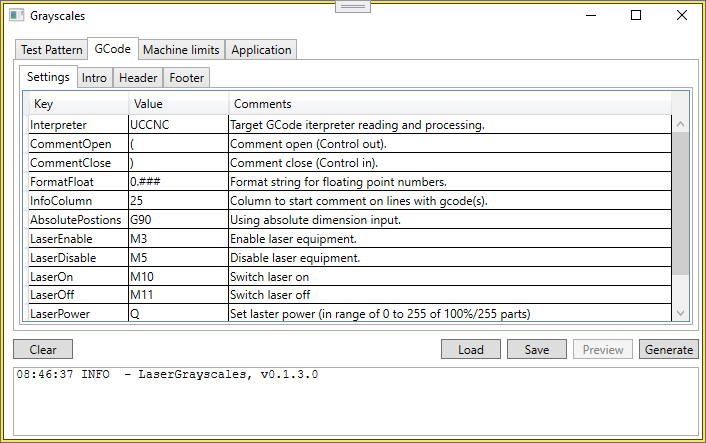
\includegraphics[width=0.8\linewidth]{./images/GCode-Settings.png}
\end{figure}

With the `GCode' tab you can specifiy all gcode specific settings depending on your gcode interpreter, that is `actual code' to use and the Intro/Header/Footer to use with
each test. (The setting for `G0 F speed of travel' is part of the test pattern settings, see \nameref{TestPatternSettingsTab})

\subsection{The Settings sub tab}\label{GCodeSettingsTab}

This sub tab give you full control over the actual GCode that is generated in the script, with one exception. Any GCode that is used in the Intro/Header/Footer sub tabs is
not subject to the settings here. The purpose of the GCode in the configuration should be clear from the `Comments' column. See \nameref{PrinciplesOfOperation} and
\nameref{GCodeAndRs274D} for more information.

\subsection{The Intro, Header and Footer sub tabs}\label{GCodeIntroTab}
\begin{figure}[h!]
    \centering
    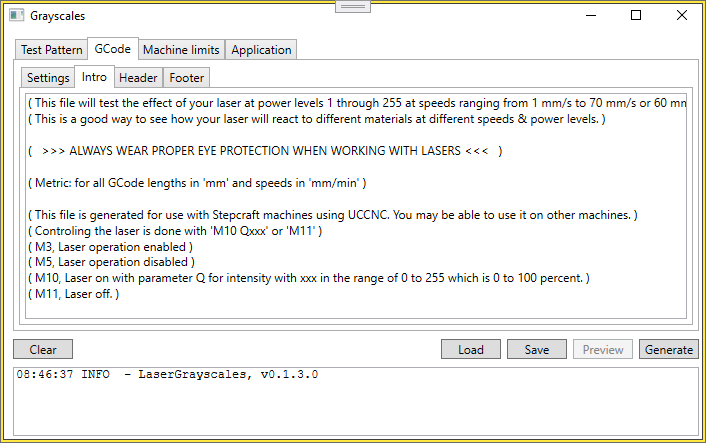
\includegraphics[width=0.8\linewidth]{./images/GCode-Intro.png}
\end{figure}

The tree sub tabs `Into', `Header' and `Footer' are identical. The first is used as an intro in the script generated where the second and last are used
as header and footer for the actions part. Each tab is free text which is copied verbatim into the script. Any GCode used is \emph{not subject to validation}.

\WarningCheckAndTest

\section{The Machine tab}\label{MachineTab}
\begin{figure}[h!]
    \centering
    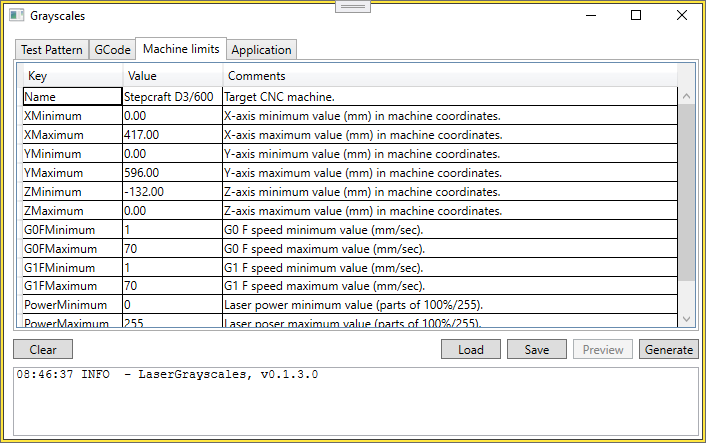
\includegraphics[width=0.8\linewidth]{./images/Machine-limits.png}
\end{figure}

The `Machine limits' tab specifies all minimum and maximum allowed values for variables used while generating a test script. This tab give you the possibility to generate
scripts wit safe and acceptable values for your machine. The purpose of the values in the configuration should be clear from the `Comments' column. See \nameref{PrinciplesOfOperation}
for more information.

\section{The Application tab}\label{ApplicationTab}
\begin{figure}[h!]
    \centering
    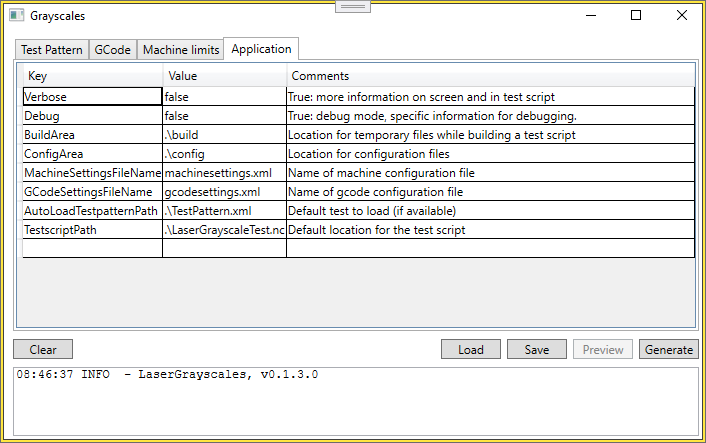
\includegraphics[width=0.8\linewidth]{./images/Application.png}
\end{figure}

The `Application' tab binds a number of items for use in the application. In general it specifies how much information to generate or where to find what kind of information.
Again, the purpose of the values in the configuration should be clear from the `Comments' column.

The application is using two (not necessarily separate) locations for configuration and building. From the configuration area two items are required, if not available
default versions are generated.

This gives you the flexibility to have configurations for several machine (or machine configurations) and several gcode interpreters available. The defaults are for
using a `Stepcraft D3/600' machine. If you for instance create a second configuration file e.g.: for `Stepcraft D2/420' you can use that too. It you use `LinuxCNC' as your
primary gcode interpreter you can use that too. Switching between configurations is now a manual action, you have to edit the `Applications' tab, which will be prone to
typing errors. In some future version a selection screen can come available but this is not yet in the planning.

It is possible to use a template `Test Pattern' that is loaded on each start. This way you are not dependent on default test pattern settings but can configure it for
your most used settings. This file is located independent from the config or build area. In some future version it may be that the last loaded or last generated pattern
will be reloaded. This is not yet available.


\begin{appendices}
    \chapter{Configuration}\label{Configuration}

The configuration\index{configuration} is done with a number files, one for test settings, one for machine settings
one for GCode settings and a general one for the application.
The files are normally located in `.\textbackslash' and are named
`testsettings.xml'\index{configuration!testsettings}\index{testsettings|see {configuration}},
`machinesettings.xml'\index{configuration!machinesettings}\index{machinesettings|see {configuration}} and
`gcodesettings.xml'\index{configuration!gcodesettings}\index{gcodesettings|see {configuration}}.
The files are readable text file (XML format) and can be looked into but it is not intended for editing.

\section{Testsettings}\index{configuration!testsettings|textbf}
This configuration file contains all default settings for a new test pattern.

\begin{tabular}{lrl}
    Name    & Default   & Description\\
    verbose & false     & if true add extra comments on the console output\\
    power minimum &   0 & default minimum laser power\\
    power maximum & 255 & default maximum laser power\\
    speed minimum &   1 & default minimum speed in mm/sec\\
    speed maximum &  70 & default maximum speed in mm/sec\\
    intro   &     GCode & default user intro section\\
    header  &     GCode & default user header section\\
    footer  &     GCode & default user footer section\\
    test script &  path & default path for test file\\
\end{tabular}

\section{Machine settings}\index{configuration!machinesettings|textbf}
This configuration file contains all machine capabilities that must be taken into account.
One is needed for validating all calculated values\index{calculated value}.

\begin{tabular}{lrl}
    Name      & Default          & Description\\
    name      & Stepcraft D3.600 & Machine name and type\\
    x minimum &                0 & minimum x value, mm in machine coordinates\\
    x maximum &              417 & maximum x value, mm in machine coordinated\\
    y minimum &                0 & minimum y value, mm in machine coordinates\\
    y maximum &              596 & maximum y value, mm in machine coordinated\\
    z minimum &             -132 & minimum z value, mm in machine coordinates\\
    z maximum &                0 & maximum z value, mm in machine coordinated\\
    speed G0 minimum &         0 & minimum speed for G0 traveling, mm/sec\\
    speed G0 maximum &        70 & maximum speed for G0 traveling, mm/sec\\
    speed minimum &            0 & minimum speed for G1, mm/sec\\
    speed maximum &           70 & maximum speed for G1, mm/sec\\
    power minimum &            0 & minimum laser power, parts $100\%/255$\\
    power maximum &          255 & maximum laser power, parts $100\%/255$\\
\end{tabular}

\section{GCode settings}\index{configuration!gcodesettings|textbf}
This configuration file contains all capabilities of the CCode interpreter.
One is needed for generating\index{operation!generator} the correct G-code.

\begin{tabular}{lrl}
    Name          & Default & Description\\
    name          &   UCCNC & Name of the G-code interpreter\\
    comment open  &       ( & Comment open character\\
    comment close &       ) & Comment close character (if empty: end of line)\\
    double format &   0.000 & floating point format\\
    info column   &      25 & Comment column on lines combining GCode with comment\\
    laser enable  &      M3 & GCode to enable laser equipment\\
    laser disable &      M5 & GCode to disable laser equipment\\
    laser on      &     M10 & GCode to switch the laser on\\
    laser off     &     M11 & GCode to switch the laser off\\
    laser power   &       Q & GCOde to set laser power\\
\end{tabular}

\section{Application settings}\index{configuration!application settings|textbf}
This configuration file binds all information from several sources together. The default paths are relative against the executable location.

\begin{tabular}{lrl}
    Name          & Default & Description\\
    Verbose       & false   & True: more information on screen and in test script\\
    Debug         & false   & True: debug mode, specific information for debugging\\
    BuildArea     & .\textbackslash{}build\textbackslash{} & Location for temporary files while building a test script\\
    ConfigArea    & .\textbackslash{}config\textbackslash{} & Location for configuration files\\
    MachineSettingsFileName & machinesettings.xml & Name of machine configuration file\\
    GCodeSettingsFileName & gcodesettings.xml & Name of gcode configuration file\\
    AutoLoadTestpatternPath & .\textbackslash{}TestPattern.xml & Default test to load (if available)\\
    TestscriptPath & .\textbackslash{}LaserGrayscaleTest.nc & Default location for the test scrip\\
\end{tabular}

    \chapter{G-Code and RS274-D}\label{GCodeAndRs274D}

G-Code and its use did not just happen `at once', Wikipedia have an informative page about \href{https://en.wikipedia.org/wiki/G-code}{G-code}
and the phrase \emph{`G-code has many variants'} in the first paragraph informs you that there is much to say
about it. The G-code that your machine is using might be a slightly different variation to the G-code that your
tool is generating (and \GS\ for that). In this chapter the general structure and some of the differences and pitfalls are discussed.

The RS274-D\index{RS274-D}\ document was approved in feb 1979 by the `Electronic Industries Association' (EIA)\index{EIA}.
Unfortunately a few subjects are mentioned but not defined or explained. Some subjects, such as a subroutine mechanism,
are not mentioned explicitly and industry is using a `post processing' phase to handle specific manufactured specifics.
By now the RS274-D has 40 years of history and still is the document referred to for G-Code compliance.

The following information about the RS274 is \emph{informative only} to give some additional insights in the use
of G-code and should not be used for design decisions. The ultimate source of information for such decisions is
the documentation with the equipment/software processing the actual G-Code.

\section{G-Code data structure}
G-code can be preceded with a line ending with a 'Start of Program'\index{Start of Program} or
'\%'\index{\%|see {Start of Program}} character.
This character can appear only once, at the end of the line. No lines preceding the line with 'Start of Program' are allowed.

G-code is defined as variable blocks of data with a `End of Block' (EOB) marker. Notably, the first block\index{block} should
be preceded by a EOB marker. Each block is a variable number of words. `End of Block' is a \grammarnl.

Words\index{word} are the actual G-code items you can recognise such as `G0', `X 123' and alike. The length (in characters) is
not fixed and there are several groups such as `Dimensional words', `Non-dimensional words' and subgroups.

The state machine handling blocks of date will, for words not sent in a block, substitute the value from the previous
block e.g: The state machine on processing block `G1 X1, Y2' will move to x=1 and y=2. On the next block `G1 Y3' the
state machine will substitute the value of 1 for x and move to x=1 and y=3.

The thing to remember is that a block of G-code words is one line of text e.g.: `G90\grammarnl' or
`G00~X0~Y0~F4200\grammarnl' are two blocks and each one is a set of words applied at the same time.

Also whitespace (spaces, tabs) have no meaning and nothing is said about lower case or upper case.
`g0\textvisiblespace{}x\textvisiblespace{}+0.0\textvisiblespace{}y\textvisiblespace{}+0.0\textvisiblespace{}f\textvisiblespace{}4200\grammarnl'
is identical to `G00X0000Y0000F4200\grammarnl'. Whitespace is used only for readability, numeric value specifications allow
for leading and trailing zero's (for dimensional values).

Comment\index{comment} text in G-Code is not explicit provided for in the RS274 except for a few odd remarks without
further explanations.

The character `)'\index{comment!)}\index{)|see {comment}} is defined as `Control In' and
`('\index{comment!(}\index{(|see {comment}} is defined as
`Control Out'. What the exact function is of these two is not explained but the general interpretation looks to be
`On Control In all following input characters is forwarded to the state machine handling blocks of data' and
`On Control Out all following input characters up to the next newline or On Control In character is ignored and not
forwarded to the state machine'. Effectively, any text between `(' and `)' (or the next \grammarnl) is ignored giving one
way of adding comments to a G-code file.

The character `\slash'\index{comment!\slash}\index{\slash|see {comment}} is defined as `Block Deleter (slash)' and
can appear as the first (non-white) character on a line. It is intended to quickly disable blocks without removing it. Effectively, any line starting with `\slash' is not processed giving another way of adding comment to a G-code file.

The character `!'\index{comment!$^^21$}\index{$^^21$|see {comment}} is used as `Start of Comment' by some C-Code interpreters. The RS274 does not
mention this character.

This depend on how the g-code interpreter is reading the file, test before you use it.

\section{Backus-Naur form}
This section can be skipped, it provides a more strict definition of G-code but does not introduce anything new to
the previous section. A more formal notation of the G-Code data in
\href{https://en.wikipedia.org/wiki/Backus%E2%80%93Naur_form}{Backus-Naur form} is given below. It does not represent
all the details in RS274 because it is composed without the use or Backus-Naur forms in mind making it hard to capture
some details.

All dimensional words (see below) should appear `in order'. That is not covered in the description below, other than
a remark, to keep the description reasonable short. Words of any type shall only appear once in a block. This is not
reflected in the grammar below, it will complicate the grammar considerable. Also the fact that missing words are
allowed in which case the state machine is substituting the value from the previous block is not represented  to keep
the grammar short and readable.
\begin{grammar}
    <gcode>      ::= <prog start> <EOB> <blocks>

    <prog start> ::= <empty> \textbar\ <any> <SOP>

    <blocks>     ::= <empty> \textbar\ <block> <blocks>

    <block> ::= <N word>\index{block}\\
                     <G words>\\
                     <dimension words>\\
                     <interpolation parameter words>\\
                     <F word>\\
                     <S word>\\
                     <T word>\\
                     <M words>\\
                     <EOB>

    <N word>     ::= `N' INTEGER\index{word}

    <G words>    ::= <empty> \textbar\ `G' <word part> <G words>

    <dimension word> ::= <dimension address> <value> <optional F word>

    <dimension address> ::= ~\\`X'\textbar `Y'\textbar `Z'\textbar `U'\textbar `V'\textbar `W'\textbar `P'\textbar `Q'\textbar `R'\textbar `A'\textbar `B'\textbar `C'\textbar `D'\textbar `E' \\// appearing in this order.

    <interpolation parameter words> ::= <interpolation address> <word part>

    <S word> ::= `S' <word part>

    <T word> ::= `T' <word part> <optional D word>

    <F word>     ::= `F' <value>

    <M words>    ::= <empty> \textbar\ `M' <word part> <M words>


    <value>      ::= REAL \textbar\ INTEGER

    <word part>  ::= <sequence number> <preparatory function number>


    <any>    ::= [\^{}\%\textbackslash n]*

    <SOP>    ::= `\%'

    <EOB>    ::= `\textbackslash n'
\end{grammar}


    \chapter{Versions}\label{Versions}

Version numbering in major . minor . build [ . bugfix ]

Even minor numbers are stable versions, odd minor number are development versions.
While in `beta' only development versions are released.

\begin{itemize}
    \item v0.3 beta, 14 dec 2024.\\
        \GS\ using an operator/image model for generating test scripts.
        All configuration settings editable in the main screen (using different tabs).
        Can save/load configuration to/from user selectable loacations.
        Can save generated test scripts to user selectable locations.
        Documentation in pdf form.
    \item v0.1.2 beta, 21 oct 2024.\\
        \GS\ added console like reporting block.
        Documentation updated.
    \item v0.1.1 beta, 17 oct 2024.\\
        \GS\ minimal functionality and documentation available.
        Can edit intro/header/footer in view Added safe-file selector.
        Generator button disabled if confuration is not valid.
    \item v0.1 beta, 14 oct 2024.\\
        \GS\ minimal functionality and documentation available.
\end{itemize}

\end{appendices}\backmatter%
    % bibliography, glossary and index would go here.
    \clearpage\addcontentsline{toc}{chapter}{Index}\printindex
\end{document}